\chapter{Evaluation}
\section{Correctness of algorithms}
The correctness of the parsing, matching, and verification algorithms are verified using unit tests. Some test cases are based on subsets of the pre-defined proof systems---natural deduction, Curry type assignment for the lambda calculus, and the sequent calculus system LK---while other test cases are based on variously modified rules from these systems and designed to catch edge cases. Some test cases based on the lambda calculus are taken from the course notes for the Type Systems module at Imperial \cite{van-bakel:2022}. Some test cases based on the system LK are taken from a set of online logic notes \cite{sequent}.

There is a high degree of confidence in the matching and verification algorithms, since they are based on custom data structures independent of the user input. To identify further edge cases in the parsing algorithm and determine how well the parsing algorithm adapts to a wide range of user inputs, the parsing algorithm is tested against extensions of the pre-defined systems and brand new proof systems.

\subsection{Lambda calculus with pairs}
\label{evaluation:lambda-pairs}
The syntaxes of $\lambda$-terms and Curry types are extended with the following constructors \cite{van-bakel:2022}:
\begin{align*}
    M, N &\Coloneqq \ldots \alt \langle M, N \rangle \alt \textsf{left}(M) \alt \textsf{right}(M) \\
    A, B &\Coloneqq \ldots \alt (A \times B)
\end{align*}
The three new constructors for $\lambda$-terms are accompanied with the following extensions to the type assignment rules:
\[
    (\textit{Pair}): \frac{\Gamma \vdash M: A \quad \Gamma \vdash N: B}{\Gamma \vdash \langle M, N \rangle: (A \times B)} \quad (\textsf{left}): \frac{\Gamma \vdash M: (A \times B)}{\Gamma \vdash \textsf{left}(M): A} \quad (\textsf{right}): \frac{\Gamma \vdash M: (A \times B)}{\Gamma \vdash \textsf{right}(M): B} 
\]
Although the user can type ``left'' and ``right'' for the two constructors, they will be rendered in math mode in \LaTeX{} as $left$ and $right$, which do not look the nicest. Prior to testing with the lambda calculus with pairs, the parsing algorithm can only handle \LaTeX{} commands that do not take any arguments, such as ``\textbackslash Gamma'' for $\Gamma$ and ``\textbackslash varphi'' for $\varphi$. The lambda calculus with pairs motivates extending the parsing algorithm to parse \LaTeX{} commands as literal strings. In this case, ``\textbackslash textsf{left}(M)'' should be rendered as $\textsf{left}(M)$ and parsed into \lstinline{Token}s as
\begin{center}
    \lstinline|[Terminal("\textsf{left}"), Terminal("("), NonTerminal(...), Terminal(")")]|
\end{center}
A correct derivation using all three newly added constructors and type assignment rules is shown in \Cref{fig:lambda-with-pairs}.
\begin{figure}[!htbp]
    \centering
    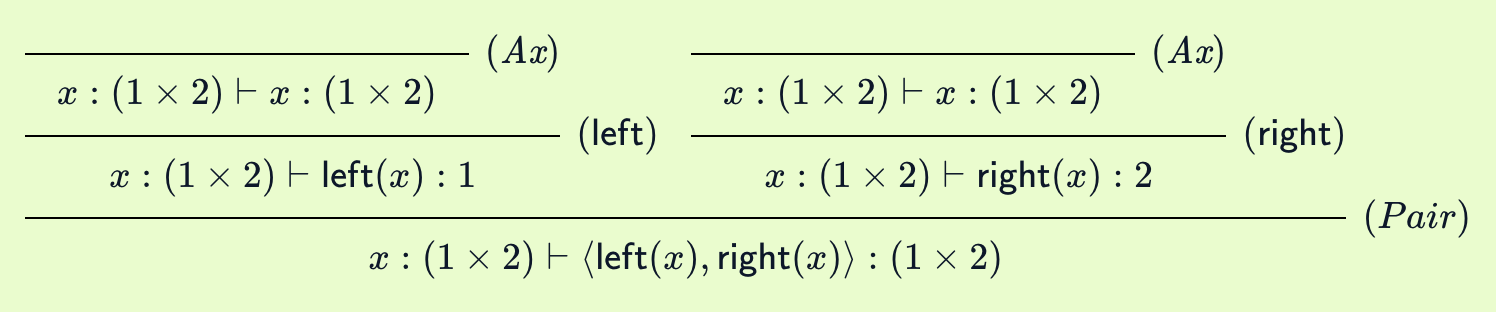
\includegraphics[width=0.7\textwidth]{evaluation/lambda-with-pairs.png}
    \caption{A correct derivation }
    \label{fig:lambda-with-pairs}
\end{figure}

\subsection{\texorpdfstring{\lbm{}}{Lambda bar mu}}
The calculus \lbm{} as presented by Curien and Herbelin \cite{curien-herbelin:2000} defines three types of terms \cite{van-bakel:2024}:
\begin{align*}
    c &\Coloneqq \langle t | e \rangle &(\textit{commands}) \\
    t &\Coloneqq x \alt (\lambda x. t) \alt (\mu \beta. c) &(\textit{terms}) \\
    e &\Coloneqq \alpha \alt (t \cdot e) \alt (\tilde{\mu}x. c) &(\textit{environments})
\end{align*}
where $x$ can be any symbol from an infinite list of term variables $a, b, c, \ldots, x, y, z \ldots$. \todo{What are $\alpha$ and $\beta$?} \lbm{} defines three kinds of statements, each typing a different syntactic category:
\begin{align*}
    \text{Statement} \Coloneqq{} &c: \Gamma \vdash \Delta &(\textit{commands}) \\
    |\  &\Gamma \vdash t: A \alt \Delta &(\textit{terms}) \\
    |\  &\Gamma \alt e: A \vdash \Delta &(\textit{environments})
\end{align*}
where $A$ represents a Curry type, while $\Gamma$ and $\Delta$ represent a set of variable type assignments. The type assignment rules are defined as follows:
\[
    (\textit{cut}): \frac{\Gamma \vdash t: A \alt \Delta \quad \Gamma \alt e: A \vdash \Delta}{\langle t|e \rangle: \Gamma \vdash \Delta}
\]

\begin{center}
    \begin{minipage}{.4\textwidth}
        \begingroup
        \addtolength{\jot}{1em}
        \begin{align*}
            (Ax_R)&: \frac{}{\Gamma, x: A \vdash x: A \alt \Delta} \\
            (\to R)&: \frac{\Gamma, x: A \vdash t: B \alt \Delta}{\Gamma \vdash (\lambda x. t): (A \to B) \alt \Delta} \\
            (\mu)&: \frac{c: \Gamma \vdash \alpha: A, \Delta}{\Gamma \vdash (\mu \alpha. c): A \alt \Delta}
        \end{align*}
        \endgroup
    \end{minipage}%
    \begin{minipage}{.4\textwidth}
        \begingroup
        \addtolength{\jot}{1em}
        \begin{align*}
            (Ax_L)&: \frac{}{\Gamma \alt \alpha: A \vdash \alpha: A, \Delta} \\
            (\to L)&: \frac{\Gamma \vdash t: A \alt \Delta \quad \Gamma \alt e: B \vdash \Delta}{\Gamma \alt (t \cdot e): (A \to B) \vdash \Delta} \\
            (\tilde{\mu})&: \frac{c: \Gamma, x: A \vdash \Delta}{\Gamma \alt (\tilde{\mu}x. c): A \vdash \Delta}
        \end{align*}
        \endgroup
    \end{minipage}
\end{center}

\section{User experience}
Three students who took the Type Systems module in autumn 2024 were invited to test the web application. User testing was conducted one-on-one over a video call. The users were asked to share their screens so that their interactions with the web application could be observed and analysed.

At the beginning of each session, the users were all told two things: that the web application supported \LaTeX{} input, and that full bracketing was necessary. Afterwards, they were given minimal guidance and navigated the web application mostly on their own, except when they did not know certain \LaTeX{} syntax or had questions about the application.

\subsection{User testing tasks}
The users were asked to complete three tasks: the first task involves deriving a conclusion in the Curry type assignment system for the lambda calculus, the second task involves extending the lambda calculus and the Curry type assignment system, and the third task involves deriving a conclusion in the system \textsc{lk}.

\subsubsection{Curry type assignment system for the lambda calculus}
In this task, the user is asked to derive the conclusion
\[
    \varnothing \vdash ((\lambda x. x)(\lambda y. y))
\]
in the Curry type assignment system using the web application. This particular conclusion is chosen because it is fairly simple and its derivation requires all three type assignment rules $(Ax)$, $(\to I)$, and $(\to E)$.

This task serves as a gentle introduction to the web application. The user only needs to focus on navigating the derivation building part of the web application and not other features, e.g. the syntax and inference rule editors. This task also serves as a quick refresher on building derivation trees, since the user testing was done around half a year after the Type Systems module had ended.

The goal of this task is to evaluate the intuitiveness of the derivation building part of the web application. In particular, the evaluation focuses on how confident the users can input conclusions, rule names, and add premises without guidance, as well as the usefulness of the error messages when the user provides an incorrect derivation.

\subsubsection{Lambda calculus with pairs}
In this task, the user is asked to extend the syntax of $\lambda$-terms and type assignment rules with pairs, as described in \Cref{evaluation:lambda-pairs}. Afterwards, the user is asked to derive the following conclusion:
\[
    x: (1 \times 2) \vdash \langle \textsf{left}(x), \textsf{right}(x) \rangle: (1 \times 2)
\]
This particular conclusion is chosen because it is fairly simple and its derivation uses all three newly added type assignment rules.

The goal of this task is to evaluate the intuitiveness of the syntax and inference rule editors. In particular, the evaluation focuses on how the users interact with the user interface to check the correctness of their definitions and the usefulness of the error messages and warnings.

\subsubsection{Sequent calculus system \textsc{lk}}
In this task, the user is asked to derive the following conclusion in the system \textsc{lk}:
\[
    ((x \lor y) \to z) \vdash (x \to z)
\]
This particular conclusion is chosen because its derivation requires the rule
\[
    (\to L): \frac{\Gamma \vdash A, \Delta \quad \Sigma, B \vdash \Pi}{\Gamma, \Sigma, (A \rightarrow B) \vdash \Delta, \Pi}
\]
which may appear quite complicated to users unfamiliar with the system \textsc{lk}, as they would need to pattern match numerous placeholders.

The goal of this task is to evaluate the usefulness of the error messages in the derivation tree and the rule viewers in guiding the users to build a correct derivation in an unfamiliar proof system.

\subsection{User testing findings}
\subsubsection{Redundant parentheses around rule names}
One user asked whether parentheses were needed around the rule names, since there was no indication from the rule name inputs and parenthesised rule names are normally expected in handwritten derivations. The user only realised parentheses were not necessary after he typed the rule name with parentheses, clicked away from the input, and saw the \LaTeX{} display added an extra set of parentheses, as in \Cref{fig:evaluation:rule-name}.

% https://tex.stackexchange.com/questions/218378/forcing-subfigures-to-have-same-height-and-take-overall-x-of-linewidth-in-latex
\begin{figure}[!htbp]
    \sbox\twosubbox{%
    \resizebox{\dimexpr\textwidth-1em}{!}{%
        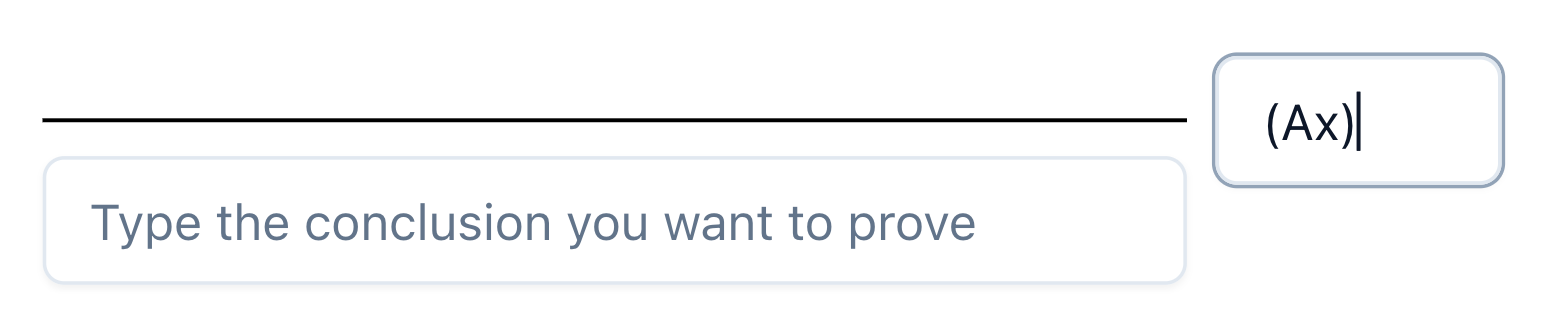
\includegraphics[height=3cm]{evaluation/rule-name-input.png}%
        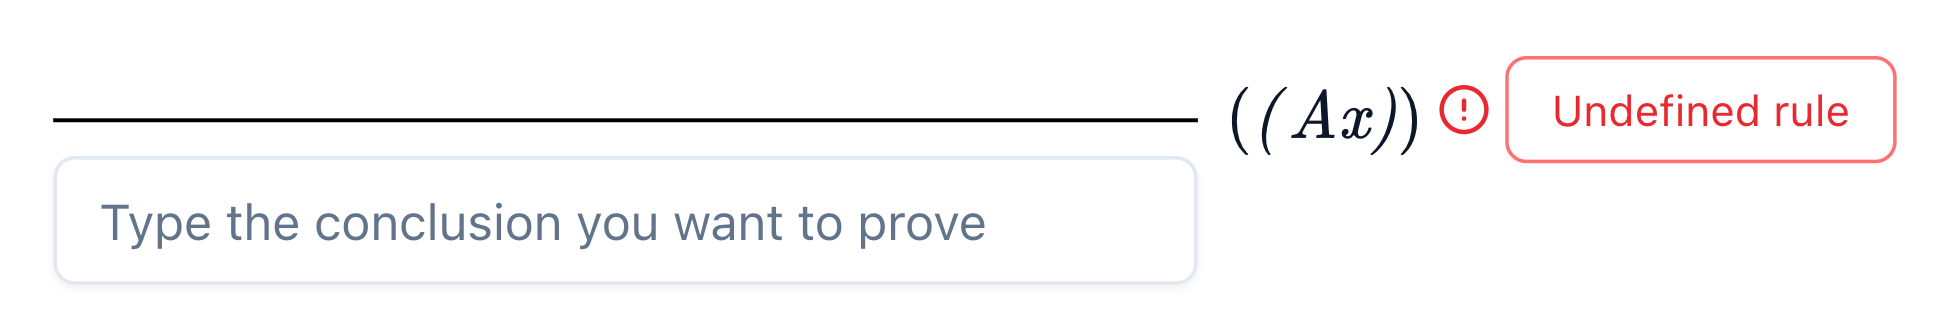
\includegraphics[height=3cm]{evaluation/rule-name-latex.png}%
    }%
    }
    \setlength{\twosubht}{\ht\twosubbox}

    \centering

    \subcaptionbox{There are no parentheses around the rule name input.}{%
        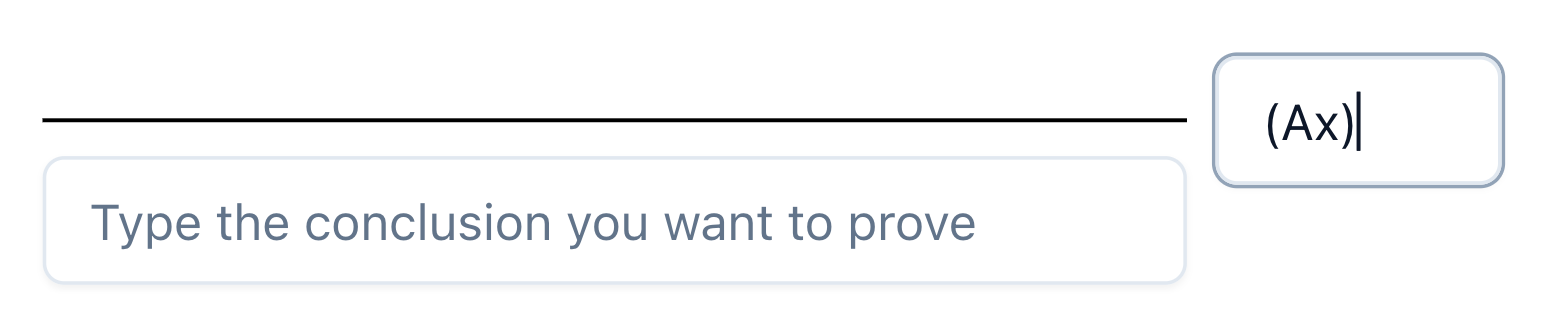
\includegraphics[height=\twosubht]{evaluation/rule-name-input.png}%
    }\quad
    \subcaptionbox{The \LaTeX{} display adds parentheses around the rule name. Note the generic ``undefined rule'' error provided.}{%
        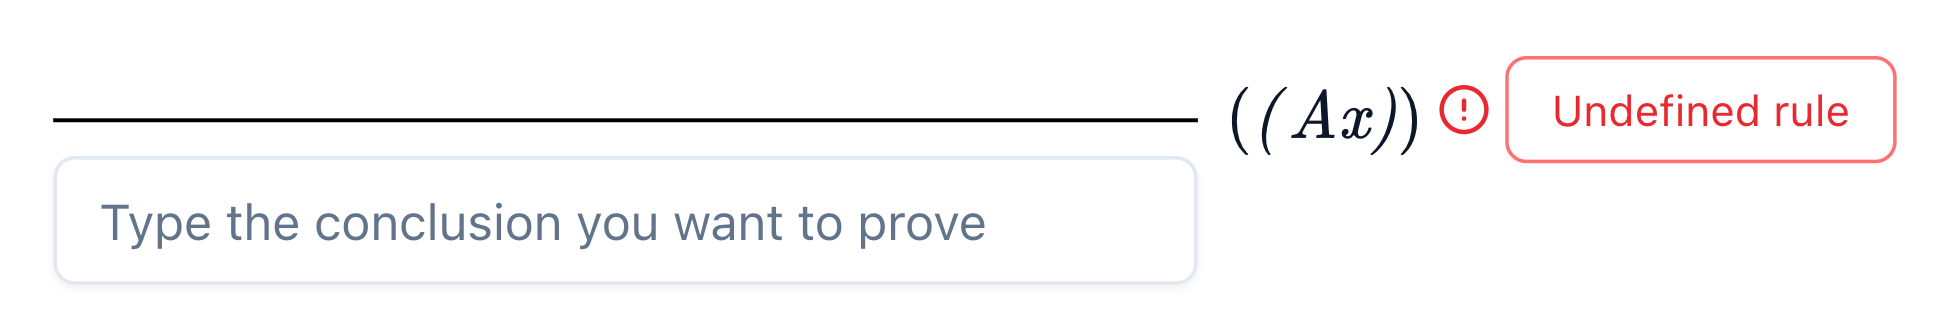
\includegraphics[height=\twosubht]{evaluation/rule-name-latex.png}%
    }
    \caption{It was unclear whether parentheses were needed around the rule name.}
    \label{fig:evaluation:rule-name}
\end{figure}

The solution is to both add an entry to the syntax guide and to display a specific error message when superfluous parentheses were added around the rule name input.

\subsubsection{Redundant parentheses around multiset terms}
All users asked whether parentheses were needed around multisets and individual multiset elements, such as $x:1, y:2$ versus $(x:1), (y:2)$ and $(x:1, y:2)$. The question may be common because in the Type Systems module and logic modules in the previous years, students were taught the bracketing conventions and operator associativity of $\lambda$-terms, Curry types, and logical connectives, but never explicitly the bracketing conventions of multisets, which were only introduced in the Type Systems module. Indeed, there was no need to formally introduce bracketing conventions for multisets in the Type Systems module since all derivations were handwritten and there was never any ambiguity when writing multisets in any of the proof systems introduced in the module.

\subsubsection{Unclear indication of correct derivations for colour-blind users}
One user with red-green colour blindness said it took multiple attempts to confirm whether his derivation was correct because the change in background colour from white to pale green appeared quite subtle to him. A comparison between the pale green background colour and a simulated version of what a green-blind user sees is shown in \Cref{fig:evaluation:colour-blind}.

\begin{figure}[!htbp]
    \centering
    \begin{subfigure}{.48\textwidth}
        \centering
        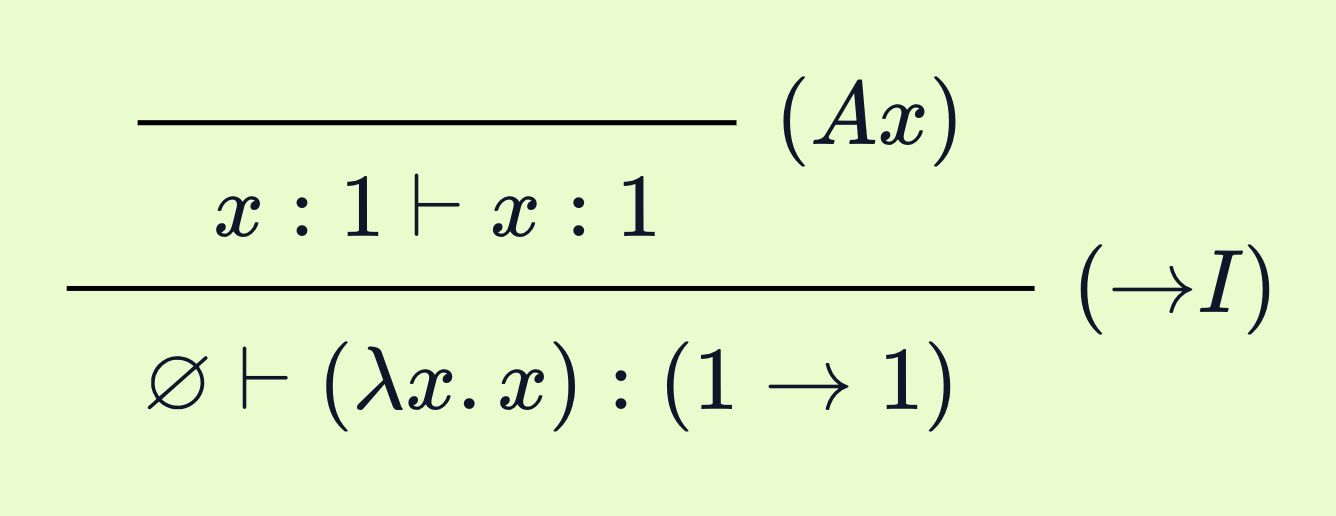
\includegraphics[width=\textwidth]{evaluation/background-normal.png}
        \caption{Pale green background colour}
    \end{subfigure}%
    \quad
    \begin{subfigure}{.48\textwidth}
        \centering
        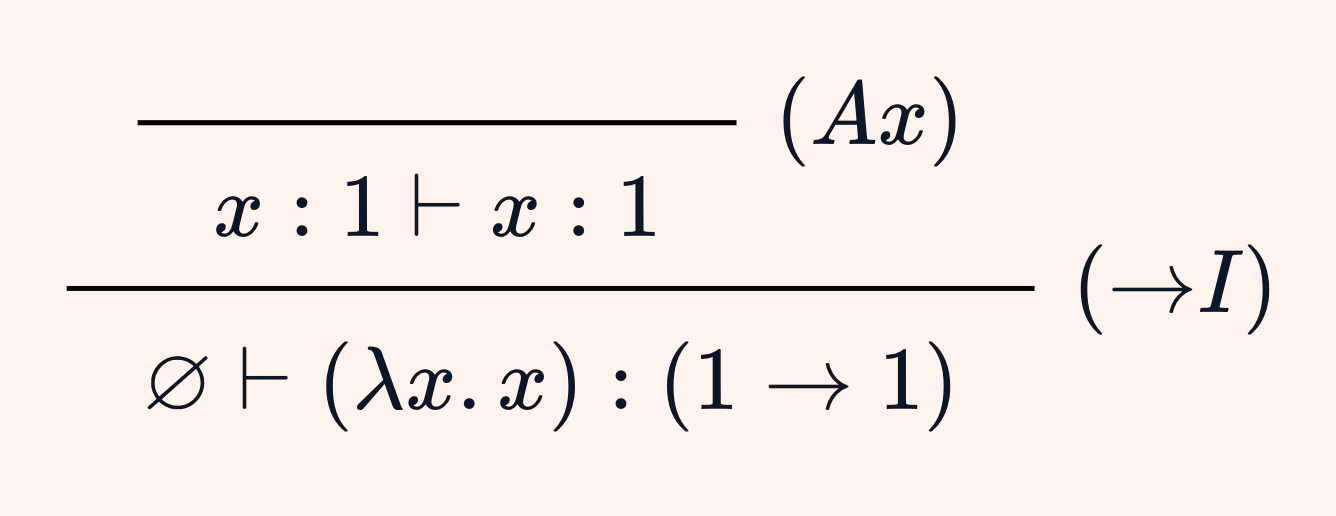
\includegraphics[width=\textwidth]{evaluation/background-colour-blind.jpg}
        \caption{Simulated view of a green-blind user}
    \end{subfigure}
    \caption{What a green-blind person sees when the background colour changes to pale green}
    \label{fig:evaluation:colour-blind}
\end{figure}

The solution is to display additional visual cues, such as a toast, that alert the user when their derivation is correct.

\subsubsection{Mistakenly typing a statement into a rule name input}
Two users mistakenly typed the conclusion of the second premise of a rule into the input for the rule of the first premise, as illustrated in \Cref{fig:evaluation:wrong-premise-input}.

\begin{figure}[!htbp]
    \centering
    \begin{subfigure}{\textwidth}
        \centering
        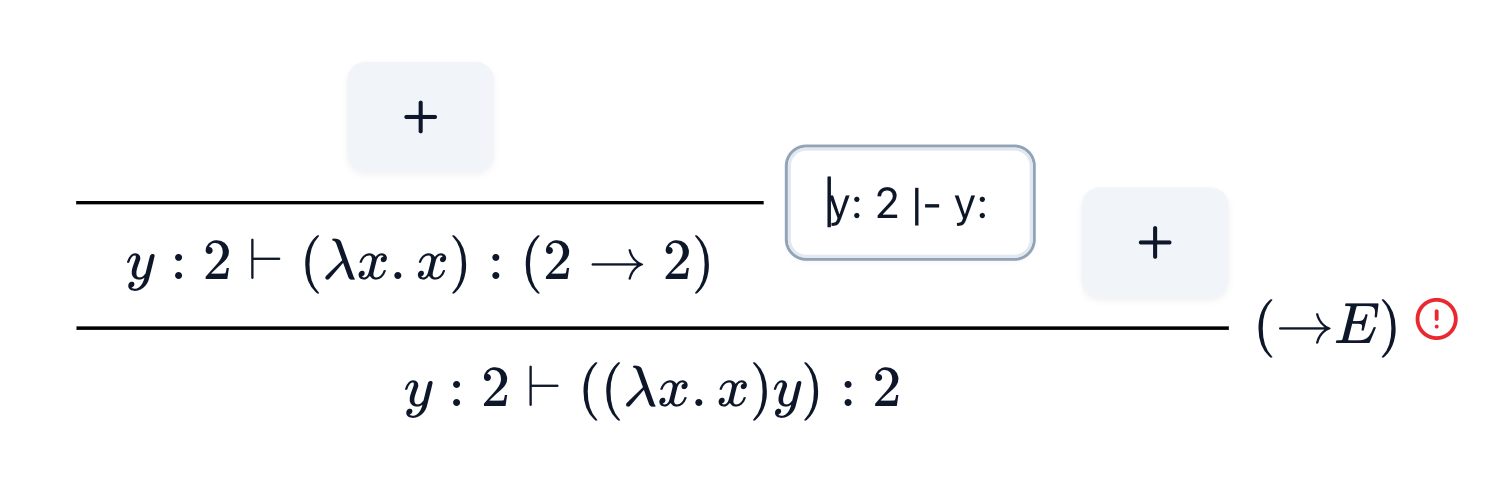
\includegraphics[height=2.5cm]{evaluation/premise-input-wrong.png}
        \caption{The user typed the conclusion instead of the rule name.}
    \end{subfigure}%
    \newline
    \begin{subfigure}{\textwidth}
        \centering
        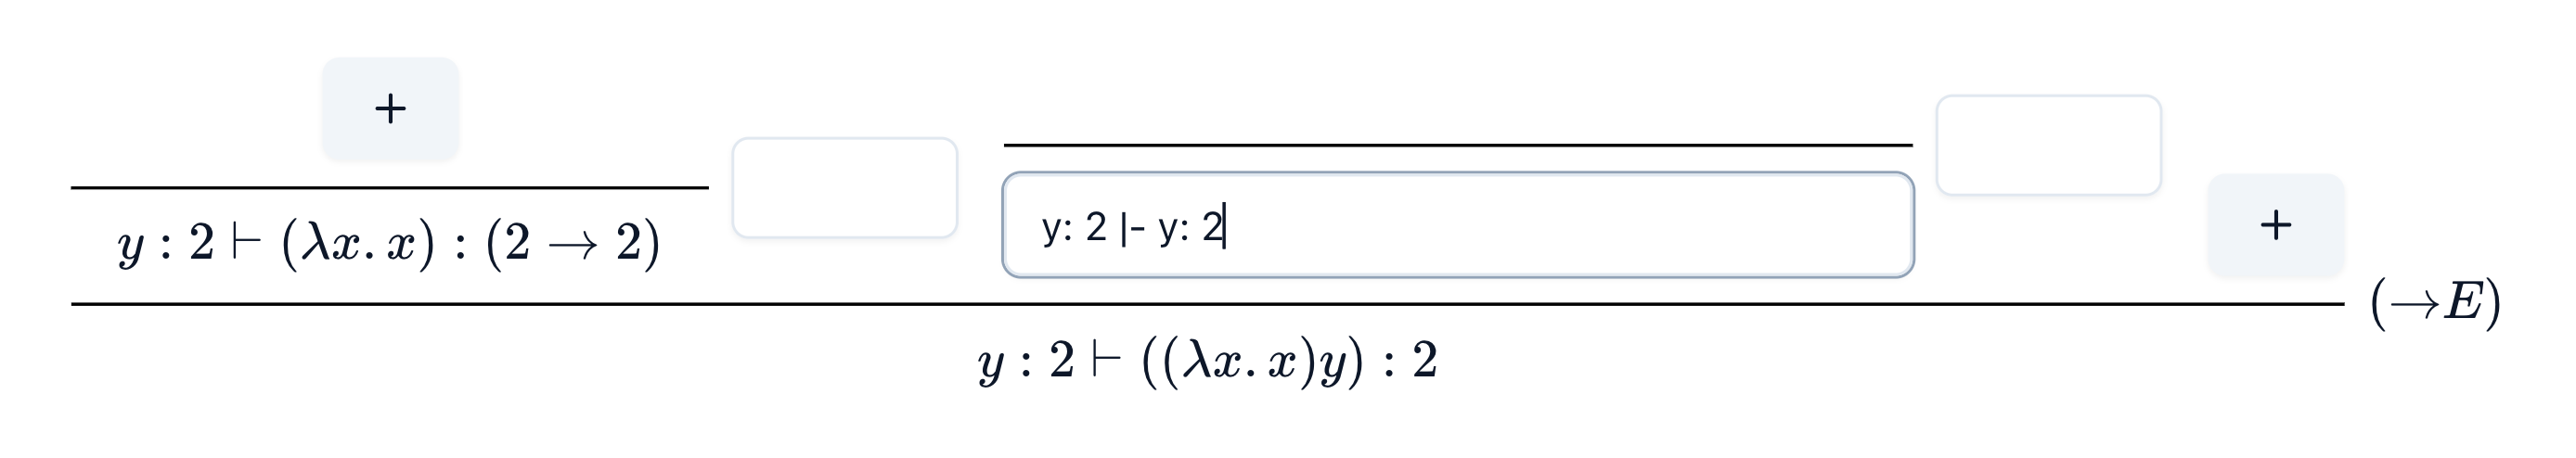
\includegraphics[height=2.5cm]{evaluation/premise-input-correct.png}
        \caption{The user should have added a new premise before typing the conclusion.}
    \end{subfigure}
    \caption{Two users mistakenly typed the conclusion of the second premise of a rule into the input for the rule of the first premise.}
    \label{fig:evaluation:wrong-premise-input}
\end{figure}

At the time of testing, there were only placeholders for the conclusion and rule name inputs at the root of the tree: the expectation was that once users input the first conclusion and rule name, they should be able to navigate the rest of the derivation tree without additional guidance. However, user testing showed otherwise. The solution was to add placeholders for all inputs in the derivation tree to indicate whether it should be a conclusion or a rule name.

\subsubsection{Displaying parsing errors before rules are specified}
When completing the first user testing task, one user inputted all conclusions of the tree before inputting the rule names. Since the web application only displayed errors when the user has specified the rule at the time of testing, the user received no feedback on syntactically incorrect inputs when inputting the conclusions and only received multiple error messages once he started typing the rule names.

The solution is to display two types of errors: general errors regardless of whether the user has specified a rule, and additional specific errors when the user has specified a rule. General errors are displayed when the user inputs a syntactically incorrect statement. Specific errors are displayed when the user inputs a syntactically correct statement which is not compatible with the structure of the corresponding inference rule statement, such as when a multiset element with a certain structure cannot be found in the user input, or if some names are incompatible.

\subsubsection{Persisting rules and derivations across reloads}
Two users accidentally closed the tab for the web application during the second task, which required extending the syntax and inference rules. When they opened the application again, the rule definitions and derivation tree were reset since data was not persisted across reloads. Although the users could quickly re-input the rules in this case, it may be more frustrating in other cases when the user accidentally closes the page when defining larger and more complicated proof systems.

The solution is to encode the definitions of the syntax and inference rules as query parameters in the URL and use the \lstinline{localStorage} property \cite{localstorage} to persist derivations across reloads. Though it is possible to store the rule definitions in \lstinline{localStorage} as well, the query parameters are already used to relay information about the rule definitions from the landing page to the derivation builder page. Suppose the rule definitions are only persisted in \lstinline{localStorage}. When the user chooses the pre-defined rules for the lambda calculus on the landing page, the URL query parameters encode this information and are passed to the derivation builder page, which parses the parameters and sets the rule definitions accordingly. If the user changes to those for the sequent calculus in the rule editor, then refreshes the page, the rule definitions and the query parameters become out of sync: the query parameters say the user wants to use the rules for the lambda calculus, yet the persisted rule definitions are actually those of the sequent calculus.